\section{Quantitative Results}
\label{sec:quant}
% Guideline 2.9: at least one clearly formatted table + interpretation.

\begin{table}[h]\centering
\resizebox{\linewidth}{!}{\begin{tabular}{lccccccccc}
\toprule
 & \multicolumn{3}{c}{$\mathbb{Z}_2$ (parity)} & \multicolumn{3}{c}{$\mathbb{Z}_3$ (count mod 3)} & \multicolumn{3}{c}{$S_3$ (permutations)} \\
\cmidrule(lr){2-4} \cmidrule(lr){5-7} \cmidrule(lr){8-10}
Model & 64 & 256 & 512 & 64 & 256 & 512 & 64 & 256 & 512 \\
\midrule
Transformer & 0.773 & 0.568 & 0.534 & 0.988 & 0.509 & 0.422 & 0.345 & 0.213 & 0.189 \\
SSM, $a\in(0,1)$ & 0.829 & 0.581 & 0.542 & 0.673 & 0.418 & 0.376 & 0.384 & 0.221 & 0.195 \\
SSM, $a\in(-1,1)$ & \textbf{1.000} & \textbf{1.000} & \textbf{0.998} & 0.517 & 0.381 & 0.356 & 0.418 & 0.293 & 0.230 \\
Gated DeltaNet, $\beta\in(0,1)$ & \textbf{0.998} & 0.682 & 0.590 & \textbf{0.998} & \textbf{0.656} & \textbf{0.491} & 0.451 & 0.249 & 0.208 \\
Gated DeltaNet, $\beta\in(0,2)$ & \textbf{1.000} & \textbf{1.000} & 0.991 & \textbf{0.997} & 0.640 & \textbf{0.486} & \textbf{0.999} & \textbf{0.785} & \textbf{0.509} \\
\bottomrule
\end{tabular}
}
\caption{RQ2: token accuracy on group-word state tracking. Models are trained on length 64 and tested
on 64, 256 and 512 (4$\times$ and 8$\times$ longer). Bold: best in column (within 0.005).
Chance is 0.5 / 0.333 / 0.167. Mean $\pm$ standard deviation over 3 seeds.}
\label{tab:state}
\end{table}

\begin{figure}[h]\centering
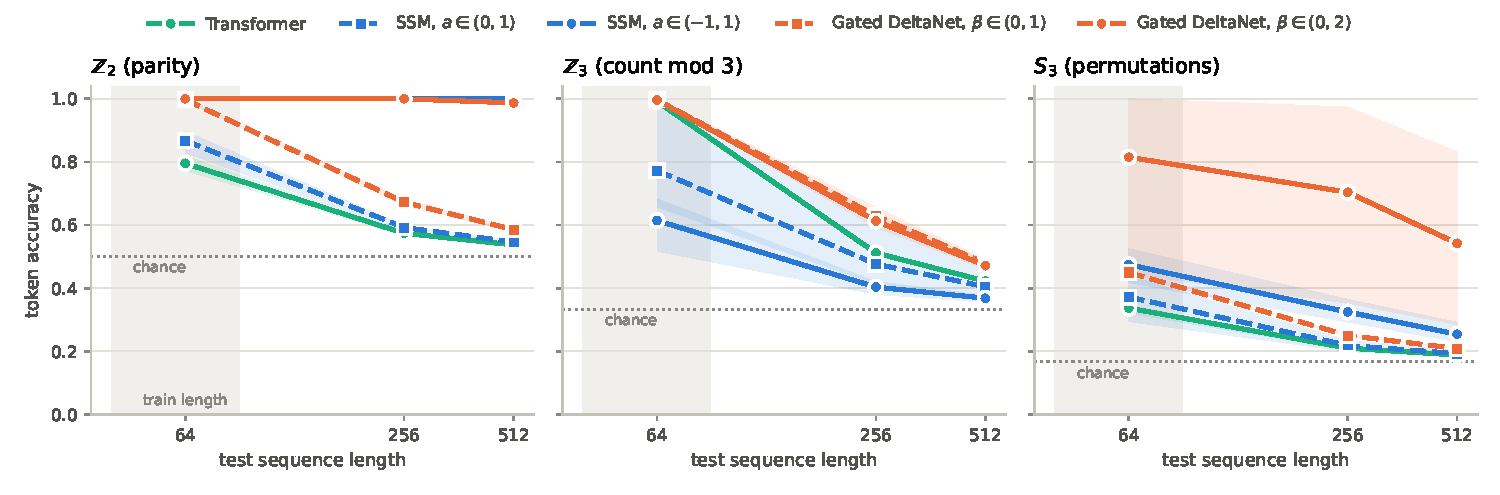
\includegraphics[width=\linewidth]{figures/state_tracking}
\caption{Length generalisation on state tracking. Colour = architecture family, line style =
eigenvalue range (dashed/square: positive only; solid/circle: extended to negative). Only models whose
transitions can represent the group keep their accuracy beyond the training length (grey band). Lines: mean over 3 seeds; shading: min--max.}
\label{fig:state}
\end{figure}

\paragraph{Beyond negative eigenvalues (RQ2b).} Table~\ref{tab:state} (bottom block) and
Fig.~\ref{fig:state-ext} add the rotational SSM and DeltaProduct$_2$.
\todo{Interpret: DeltaProduct$_2$ with $\beta\in(0,2)$ is the only model that learns $S_3$ on all 3
seeds and keeps 0.91 at 8$\times$ the training length (Gated DeltaNet: 0.54, high variance). On
$\mathbb{Z}_3$, every model that fits the training length (attention, DeltaNet, DeltaProduct, rotational
SSM: 0.97--1.00) falls to 0.43--0.52 at length 512. The rotational SSM fits $\mathbb{Z}_2$ at length 64
on only 1 of 3 seeds.}

\begin{figure}[h]\centering
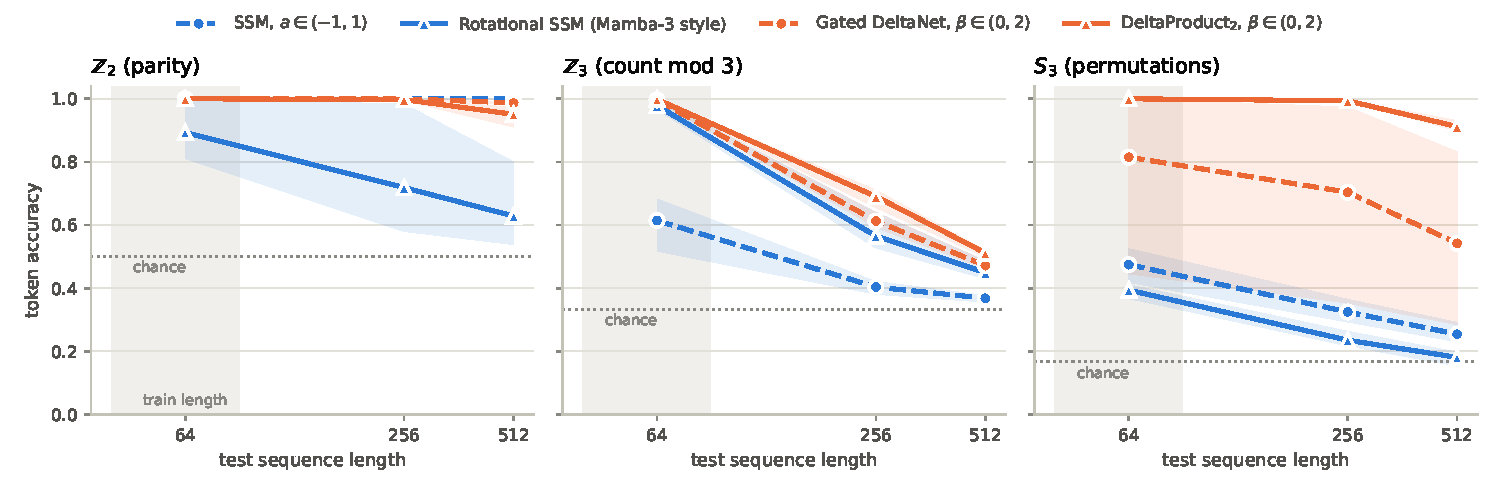
\includegraphics[width=\linewidth]{figures/state_tracking_ext}
\caption{The extensions against their predecessors (dashed). Lines: mean over 3 seeds; shading: min--max.}
\label{fig:state-ext}
\end{figure}

\begin{table}[h]\centering\small
\begin{tabular}{lccccc}
\toprule
Train length & test 16 & test 32 & test 64 & test 256 & test 512 \\
\midrule
16 & 1.000$\pm$0.000 & -- & 0.675$\pm$0.187 & 0.432$\pm$0.065 & 0.382$\pm$0.032 \\
32 & -- & 0.995$\pm$0.008 & 0.877$\pm$0.127 & 0.518$\pm$0.093 & 0.425$\pm$0.046 \\
64 & -- & -- & 0.719$\pm$0.186 & 0.453$\pm$0.081 & 0.394$\pm$0.040 \\
\bottomrule
\end{tabular}

\caption{Rotational SSM on $\mathbb{Z}_3$ trained at different lengths (mean $\pm$ std over 3 seeds).}
\label{tab:rotation-length}
\end{table}

\begin{figure}[h]\centering
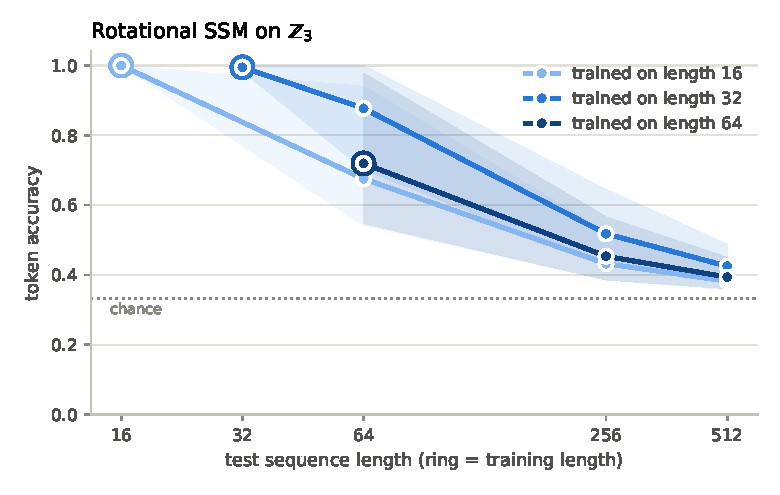
\includegraphics[width=0.6\linewidth]{figures/rotation_length}
\caption{Rotational SSM on $\mathbb{Z}_3$: accuracy vs.\ test length for three training lengths.
Ring: the training length. Shading: min--max over 3 seeds.}
\label{fig:rotation-length}
\end{figure}

\todo{Table: RQ1 MQAR accuracy vs.\ number of pairs (with state size column).}
\todo{Table: RQ3 hybrid placement.}
\todo{Table: RQ4 latency / memory / decode throughput on the RTX 4050.}
\todo{Interpret every table in prose.}
